% !TeX root=../main.tex
\chapter{روش و راه‌حل پیشنهادی}
%\thispagestyle{empty} 
\section{مقدمه}
در این فصل روش پیدا کردن علت خطا در یک برنامه‌ی توصیف شده در نت‌کت پویا توضیح داده می‌شود.
در بخش اول مدل معنایی عبارات نت‌کت پویا با در قالب ساختمان رویداد تعریف می‌شود.
در بخش دوم یک مدل علّی برای توصیف ساختمان رویداد مطرح می‌شود.
در نهایت در بخش سوم شامل استفاده از این چگونگی ترکیب این دو روش برای توضیح خطا در یک برنامه نت‌کت پویا توضیح داده می‌شود..


\section{مدل معنایی عبارات نت‌کت پویا در قالب ساختمان رویداد}
در این بخش ابتدا انواع ترکیب و محدود‌سازی ساختمان‌‌های رویداد تعریف می‌شود.
سپس با استفاده از این تعاریف  یک مدل معنایی برای عبارات نت‌کت پویا ارائه می‌شود.

\begin{definition}
    فرض کنید
    $\mr{E} = (E,\#,\vdash)$
    یک ساختمان رویداد باشد.
    به ازای یک مجموعه‌ی
    $A \subseteq E$
    ،
    محدودیت
    \lf{Restriction}
    $\mr{E}$
    به
    $A$
    یک ساختمان رویداد به شکل زیر است:
    \begin{align*}
        \mr{E} \lceil A = (A,\#_A,\vdash_A)
    \end{align*}
    که اگر 
    $Con_A$
    مجموعه‌ی تمامی زیرمجموعه‌های بدون تعارض 
    $A$ 
    در 
    $\mr{E}\lceil A$
    باشد آنگاه داشته باشیم:
    \begin{align*}
        X \subseteq Con_A & \iff X \subseteq A \wedge X \in Con                 \\
        X \vdash_A e      & \iff X \subseteq A \wedge e \in A \wedge X \vdash e
    \end{align*}
\end{definition}

\begin{definition}
    فرض کنید
    $\mr{E} = (E,\#,\vdash)$
    یک ساختمان رویداد و
    $a$
    یک رویداد باشد.
    ساختمان رویداد
    $a\mr{E} = (E',\#',\vdash')$
    که به معنای افزودن رویداد 
    $a$
    به عنوان پیشوند
    به 
    $\mr{E}$
    است
    به گونه‌ای تعریف می‌شود که داشته باشیم:
    \begin{align*}
         & E' = \s{(0,a)} \cup \s{(1,e)|e \in E},                                                                               \\
         & e_0' \#' e_1'  \iff \exists e_0,e_1.e_0' = (1,e_0)
        \ \wedge \ e_1' = (1,e_1) \ \wedge \ e_0 \# e_1                                                                         \\
         & X \vdash' e' \iff e' = (0,a) \text{ or } [e' = (1,e_1) \ \wedge \ (0,a)\in X \ \wedge \ \s{e|(1,e)\in X} \vdash e_1]
    \end{align*}
\end{definition}

\begin{definition}
    یک ساختمان رویداد برچسب‌دار
    \lf{Labeled Event Structure}
    یک پنج‌تایی به شکل
    $(E,\#,\vdash,L,l)$
    است که در آن
    $(E,\#,\vdash)$
    یک ساختمان رویداد،
    $L$
    یک مجموعه از برچسب‌ها
    (فاقد عنصر *
    \footnote{
        در ادامه از * برای مشخص کردن رویداد‌های ناهمگام استفاده می‌کنیم. به همین دلیل این عنصر را به عنوان یک برچسب خاص از مجموعه‌ی برچسب‌های ممکن کنار می‌گذاریم.
    }
    )
    و
    $l$
    یک تابع به فرم
    $l: E \ra L$
    است که به هر رویداد یک برچسب اختصاص می‌دهد.
    یک ساختمان رویداد برچسب‌دار را به اختصار به صورت
    $(\mr{E},L,l)$
    نشان می‌دهیم.
\end{definition}

\begin{definition}
    در یک ساختمان رویداد رابطه‌ی
    $\doublevee$
    را به صورت زیر تعریف می‌کنیم:
    \begin{align*}
        e \doublevee e' \iff e \# e' \vee e = e'
    \end{align*}
\end{definition}

\begin{definition}
    فرض کنید
    $(\mr{E},L,l)$
    یک ساختمان رویداد برچسب‌دار و
    $\alpha$
    یک برچسب باشد.
    $\alpha(\mr{E},L,l)$
    را به صورت یک ساختمان رویداد برچسب‌دار به شکل
    $(\alpha \mr{E},L',l)$
    تعریف می‌کنیم که در آن
    $L' = \s{\alpha}\cup L$
    و به ازای هر
    $e' \in E'$
    داشته باشیم:
    $$
        l'(e') = \begin{cases}
            \alpha & \text{ if } e = (0,\alpha) \\
            l(e)   & \text{ if } e = (1,e)
        \end{cases}
    $$
\end{definition}

\begin{definition}
    فرض کنید
    $\mr{E}_0 = (E_0,\#_0,\vdash_0,L_0,l_0)$
    و
    $\mr{E}_1 = (E_1,\#_1,\vdash_1,L_1,l_1)$
    دو ساختمان رویداد برچسب‌دار باشند.
    مجموع این دو ساختمان رویداد
    $\mr{E}_0 + \mr{E}_1$
    را به صورت یک ساختمان رویداد برچسب‌دار
    $(E,\#,\vdash,L,l)$
    تعریف می‌کنیم که در آن داشته باشیم:
    \begin{align*}
        E = \s{(0,e)|e \in E_0} \cup \s{(1,e)|e \in E_1}
    \end{align*}
    با استفاده از این مجموعه از رویداد‌ها توابع
    $\iota_k: E_k \ra E$
    را به ازای
    $k=0,1$
    به شکل زیر تعریف می‌کنیم:
    \begin{align*}
        \iota_k(e) = (k,e)
    \end{align*}
    رابطه‌ی تعارض را به گونه‌ای تعریف می‌کنیم که داشته باشیم:
    \begin{align*}
        e \# e' \iff & \exists e_0,e_0'. e = \iota_0(e_0)
        \wedge e' = \iota_0(e_0') \wedge e_0 \#_0e_0'             \\
                     & \bigvee \exists e_1,e_1'. e = \iota_1(e_1)
        \wedge e' = \iota_1(e_1') \wedge e_1 \#_1 e_1'            \\
                     & \bigvee \exists e_0,e_1.(e=\iota_1(e_0)
        \wedge e' =\iota_1(e_1)) \vee
        (e'=\iota_1(e_0) \wedge e =\iota_1(e_1))
    \end{align*}
    رابطه‌ی فعال‌سازی را به گونه‌ای تعریف می‌کنیم که داشته باشیم:
    \begin{align*}
        X \vdash e \iff & X \in Con \wedge e \in E \wedge                   & \\
                        & (\exists X_0 \in Con_0,e_0 \in E_0.X = \iota_0X_0
        \wedge e = \iota_0(e_0) \wedge X_0 \vdash_0 e_0) \text{ or }          \\
                        & (\exists X_1 \in Con_1,e_1 \in E_1.X = \iota_1X_1
        \wedge e = \iota_1(e_1) \wedge X_1 \vdash_1 e_1)                      \\
    \end{align*}
     مجموعه‌ی برچسب‌ها را به صورت
    $L = L_0 \cup L_1$
    و تابع برچسب‌گذاری را به شکل تعریف می‌کنیم:
    $$
        l(e) = \begin{cases}
            l_0(e_0) & \text{ if } e = \iota_0(e_0) \\
            l_1(e_1) & \text{ if } e = \iota_1(e_1)
        \end{cases}
    $$
\end{definition}

\begin{definition}
    فرض کنید که
    $\mr{E_0} = (E_0,\#_0,\vdash_0,L_0,l_0)$
    و
    $\mr{E_1} = (E_1,\#_1,\vdash_1,L_1,l_1)$
    دو ساختار رویداد برچسب‌گذاری شده باشند.
    حاصلضرب آن‌ها
    $\mr{E}_0 \times \mr{E}_1$
    را به صورت یک ساختمان رویداد برچسب‌گذاری شده
    $\mr{E} = (E,\#,\vdash,L,l)$
    تعریف می‌کنیم که در‌ آن رویداد‌ها به صورت زیر تعریف می‌شوند:
    \begin{align*}
        E_0 \times_* E_1 =
        \s{(e_0,*)|e_0 \in E_0}
        \cup \s{(*,e_1)|e_1 \in E_1}
        \cup \s{(e_0,e_1)| e_0 \in E_0 \wedge e_1 \in E_1}
    \end{align*}
    با توجه به این مجموعه‌ رویداد‌ها توابعی به شکل
    $\pi_i: E \ra_* E_i$
    تعریف می کنیم که به ازای
    $i=0,1$
    داشته باشیم:
    $\pi_i(e_0,e_1) = e_i$.
    در اینجا رابطه‌ی تعارض را به کمک رابطه‌ی
    $\doublevee$
    که پیش‌تر تعریف شد، به شکل زیر به ازای تمامی رویداد‌های
    $e,e' \in E$
    توصیف می‌کنیم:
    \begin{align*}
        e \doublevee e' \iff
        \pi_0(e)\doublevee_0 \pi_0(e')
        \vee \pi_1(e)\doublevee_1\pi_1(e')
    \end{align*}
    رابطه‌ی فعال‌سازی  را به صورت زیر تعریف می‌کنیم:
    \begin{align*}
         & X \vdash e \iff X \in Con \wedge e \in \mathcal{E} \wedge     \\
         & (\pi_0(e)\text{ defined } \Rightarrow \pi_0X\vdash_0\pi_0(e))
        \wedge (\pi_1(e)\text{ defined } \Rightarrow \pi_1X\vdash_1\pi_1(e))
    \end{align*}
    مجموعه‌ی برچسب‌های حاصلضرب را به صورت زیر تعریف می‌کنیم:
    \begin{align*}
        L_0 \times_* L_1 = \s{ (\alpha_0,*)|\alpha_0 \in L_0}
        \cup \s{(*,\alpha_1)|\alpha_1 \in L_1}
        \cup \s{(\alpha_0,\alpha_1)|\alpha_0 \in L_0 \wedge \alpha_1 \in L_1}
    \end{align*}
    در انتها تابع برچسب‌گذاری را به صورت زیر تعریف می‌کنیم:
    \begin{align*}
        l(e) = (l_0(\pi_0(e),l_1(\pi_1(e))))
    \end{align*}
\end{definition}

\begin{definition}
    فرض کنید که
    $\mr{E} = (E,\#,\vdash,L,l)$
    یک ساختمان رویداد برچسب‌دار باشد.
    فرض کنید
    $\Lambda$
    یک زیرمجموعه از
    $L$
    باشد.
    محدودیت
    $\mr{E}$
    به
    $\Lambda$
    را به صورت
    $\mr{E}\lceil\Lambda$
    و به شکل یک ساختمان رویداد برچسب‌گذاری شده به شکل
    $(E',\#',\vdash',L\cap\Lambda,l')$
    که در آن
    $(E',\#',\vdash') = (E,\#,\vdash)\lceil \s{e \in E|l(e)\in \Lambda}$
    است و تابع برچسب‌گذاری معادل محدودسازی تابع
    $l$
    به دامنه‌ی
    $L\cap \Lambda$
    است.
\end{definition}

\subsection{معنای عبارات نت‌کت پویای نرمال}
در ادامه ابتدا فرم نرمال عبارات نت‌کت پویا را تعریف می‌کنیم.
فرض کنید که فیلد‌های ممکن برای بسته‌ها 
$f_1,f_2,...,f_k$
باشند.
یک فیلتر کامل
\lf{Complete Test}
به صورت
$\alpha = f_1 = n_1 ... f_k = n_k$
و یک اختصاص کامل
\lf{Complete Assignment}
به صورت
$\pi = f_1 \la n_1 ... f_k \la n_k$
تعریف می‌شود.
می‌گوییم یک عبارت
$q$
در
$NetKAT^{-dup}$
به فرم نرمال است
اگر به شکل
$\Sigma_{\alpha\cdot\pi \in \mathcal{A}}\alpha\cdot\pi$
باشد که داشته باشیم
$\mathcal{A} = \s{\alpha_i\cdot\pi_i | i \in I}$.
در عبارت قبل
$I$
مدل زبانی
$NetKAT^{-dup}$
می‌باشد.
بر اساس لم ۵ در
\cite{dynetkat}
به ازای هر عبارت
$p$
در
$NetKAT^{-dup}$
یک عبارت
$p'$
به فرم نرمال وجود دارد که داشته باشیم:
$p\equiv p'$.

\begin{definition}
    فرض کنید که 
    $p$
    یک عبارت نت‌کت پویا و 
    $X$
    متغیری باشد که در 
    $p$
    استفاده شده است.
    یک رخداد 
    $X$
    در 
    $p$
    محافظت شده 
    \lf{Guarded}
    است اگر و تنها اگر یکی از شروط زیر برقرار باشد:
    \begin{itemize}
        \item $p$
         جمله‌ای به شکل 
        $p';t$
        داشته باشد که در آن 
        هیچ متغیری در 
        $p'$
        استفاده نشده باشد یا 
        $X$ 
        در 
        $t$
        رخ داده باشد و رخداد تمامی متغیر‌های دیگر در 
        $p'$
        محافظت شده باشند.
        \item عبارت 
        $p$
        به فرم یکی از عبارت‌های 
        $y?X;t$
        یا
        $y!X;t$
        باشد.
    \end{itemize}
\end{definition}

\begin{definition}
    یک عبارت نت‌کت پویا مانند 
    $p$
    را محافظت‌ شده
    \lf{Guarded}
    می‌نامیم اگر تمامی رخداد‌های تمامی متغیر‌ها در آن محافظت شده باشد.
\end{definition}

\begin{definition}
    \label{def:dynetkat-normal}
    زبان نت‌کت پویا‌ نرمال را با دستور زبان زیر تعریف می‌کنیم:
    \begin{align*}
        F ::= & \alpha\cdot\pi                                          \\
        D ::= & \bot | F;D | x?F;D | x!F;D | D \parallel D | D \oplus D
    \end{align*}
\end{definition}
با استفاده از این لم، در لم ۹ که در
\cite{dynetkat}
ثابت شده است،
به ازای هر عبارت محافظت شده 
$p$
در نت‌کت پویا یک عبارت معادل آن به فرم نرمال وجود دارد که داشته باشیم:
$p \equiv q$.
بنابراین در نهایت می‌توانیم هر عبارت محافظت شده نت‌کت پویا را به فرم یک عبارت نرمال 
با توجه به تعریف 
\ref{def:dynetkat-normal}
بنویسیم.
در ادامه فرض کنیم که
$\mc{A}$
مجموعه‌ی الفبا شامل تمامی حروف به شکل
$\alpha\cdot\pi,x?F,x!F$
باشد و داشته باشیم
$\alpha \in \mc{A}, L \subseteq \mc{A}$.
معنای عبارات نت‌کت پویای نرمال را با به صورت زیر تعریف می‌کنیم:
\begin{align*}
    \sem{\bot}              & = (\e,\e)                               \\
    \sem{\alpha;t}          & = \alpha(\sem{t})                       \\
    \sem{t_1 \oplus t_2}    & = \sem{t_1} + \sem{t_2}                 \\
    \sem{t_1 \parallel t_2} & = \sem{t_1} \times \sem{t_2}            \\
    \sem{\delta_{L}(t)}     & = \sem{t}\lceil \mathcal{A} \setminus L
\end{align*}
سمت چپ معادلات بالا عبارات نت‌کت پویای نرمال و در سمت راست ساختمان رویداد معادل هر یک مشخص شده است.
در معادلات بالا 
$(\e,\e)$
یک ساختمان رویداد که مجموعه‌ی رویداد‌ها و مجموعه‌ی برچسب‌های آن تهی است را نشان می‌دهد.

\section{مدل علی برای ساختمان رویداد}
در ادامه نحوه‌ی توصیف یک ساختمان رویداد در قالب یک مدل علی را بیان می کنیم.

فرض کنیم که
$\mr{E} = (E,\#,\vdash)$
یک ساختمان رویداد باشد.
مدل علی این ساختمان رویداد را به صورت
$\mc{M} = (\mc{s},\mc{F},\mc{E})$
تعریف می‌کنیم که در آن
$\mc{S} = (\mc{U},\mc{V},\mc{R})$.
در این مدل فرض می‌کنیم همه‌ی متغیر‌ها از نوع بولی هستند.
همچنین در این مدل متغیر برونی در نظر نمی‌گیریم بنابراین داریم
$\mc{U} = \e$.
اگر فرض کنیم مجموعه‌ رویدادها به صورت
$E = \s{e_1,e_2,...,e_n}$
باشد مجموعه‌ی متغیر‌های درونی را به صورت زیر تعریف می‌کنیم:
\begin{align*}
    \mathcal{V} = & \s{C_{e_i,e_j} |  1 \leq i < j \leq n.
    e_i \in E \wedge e_j \in E}                              \\
                  & \cup \s{EN_{s,e} | s \in \mathcal{P}(E),
    e \in E. e \not \in s }                                  \\
                  & \cup \s{M_{s,e} | s \in \mathcal{P}(E),
        e \in E. e \not \in s } \cup \s{PV}
\end{align*}
به صورت شهودی به ازای هر عضو از رابطه‌های
$\#,\vdash,\vdash_{min}$
یک متغیر درونی در نظر می‌گیریم که درست بودن این متغیر به معنای وجود عنصر منتاظر با آن در رابطه است.
به ازای
$x,y \in \mc{P}(E)$
پوشیده
شدن 
\lf{Covering}
$x$
توسط
$y$
را که با 
$x \prec y$
نمایش می‌دهیم به صورت زیر تعریف می‌کنیم:
\begin{align*}
    x \subseteq y \wedge x \neq y \wedge
    (\forall z. x \subseteq z \subseteq y \Rightarrow x = z
    \text{ or } y = z)
\end{align*}
همچنین به ازای هر متغیر 
$X \in \mc{V}$
بردار
$\vec V_X$
را بردار شامل همه‌ی متغیر‌های درونی به غیر از 
$X$
تعریف می‌کنیم.
با استفاده از این تعاریف 
توابع متغیر‌های درونی را به صورت زیر تعریف می‌کنیم:
$$
    \f{C_{e,e'}} = \begin{cases}
        true  & \text{ if } e \# e'\\
        false & \text{ otherwise }
    \end{cases}
$$
$$
    \f{M_{s,e}} = \begin{cases}
        Min(s,e) \wedge Con(s) & \text{ if } s \vdash_{min} e \\
        false                  & \text{ otherwise }
    \end{cases}
$$
\begin{align*}
    \f{EN_{s,e}} & =
    \left(
    M_{s,e} \vee
    \left(
    \bigvee_{s'\prec s}EN_{s',e}
    \right)
    \right)
    \bigwedge
    Con(s)
\end{align*}
که در آن‌ها داریم:
\begin{align*}
    Con(s)   & =   \left(
    \bigwedge_{ 1\leq j<j' \leq n \wedge e_j,e_{j'} \in s}
    \neg C_{e_j,e_{j'}}
    \right)               \\
    Min(s,e) & = \left(
    \bigwedge_{s' \subseteq E. (s' \subset s \vee s \subset s')
        \wedge e \notin s'}
    \neg M_{s',e}
    \right)
\end{align*}
فرض کنید که
$\mathbb{E}$
مجموعه‌ی تمامی سه‌تایی‌ها به فرم
$(E,\#',\vdash')$
باشد که داشته باشیم:
\begin{align*}
    \#' \subseteq E \times E \\
    \vdash' \subseteq \mc{P}\times E
\end{align*}
یک تابع به فرم
$ES: \times_{V \in \mathcal{V}\setminus \s{PV}} \mathcal{R}(V) \rightarrow \mathbb{E}$
تعریف می‌کنیم که به صورت شهودی ساختمان رویداد حاصل از مقدار فعلی متغیر‌ها در مدل علی را به دست می‌دهد.
فرض کنیم 
$\vec v$
برداری شامل مقادیر متغیرهای
$\mc{V} \setminus \s{PV}$
باشد.
به ازای هر متغیر مانند 
$V \in \mc{V}$
مقدار آن در 
$\vec v$
را با
$\vec v(V)$
نمایش می‌دهیم.
تابع 
$ES$
را به گونه‌ای تعریف می‌کنیم که اگر 
$ES(\vec v) = (E,\#',\vdash')$
آنگاه داشته باشیم:
\begin{align*}
    \forall e,e' \in E. e \#' e' \wedge e' \#' e
     & \iff \vec{v}(C_{e,e'}) = \T \\
    \forall s \in \mathcal{P}(E), e \in E.  s \vdash' e
     & \iff \vec{v}(EN_{s,e}) = \T
\end{align*}
در نهایت فرض می‌کنیم که رفتار بد سیستمی که در قالب ساختمان رویداد مدل شده است، در قالب تابع متغیر 
$PV$
توصیف شده است و در صورتی که رفتار بد در سیستم وجود داشته باشد مقدار آن درست و در غیر این صورت غلط است.
با استفاده از مدل علی که به این شکل توصیف شود برای پیدا کردن علت خطا کافی است علت واقعی 
$PV=\T$
را در مدل علی و مطابق تعریف پیدا کنیم.



\section{پیدا کردن علت خطا در نت‌کت پویا}

با استفاده از تعاریف بخش‌های قبلی در این بخش به چگونگی پیدا کردن علت خطا در یک برنامه توصیف شده در نت‌کت پویا می‌پردازیم.

فرض می‌کنیم که یک عبارت نت‌کت پویا
$p$
در اختیار داریم.
ابتدا عبارت
$p$
را به فرم نرمال مطابق تعریف 
\ref{def:dynetkat-normal}
در می‌آوریم.
فرض کنیم عبارت 
$q$
فرم نرمال
عبارت 
$p$
باشد.
اکنون فرض کنیم 
$\mr{E} = \sem{q}$
ساختمان رویداد معادل 
$q$
باشد.
اکنون مدل علّی 
$\mc{M}$
را بر اساس
$\mr{E}$
می‌سازیم و رفتار نا امن را در قالب تابع متغیر
$PV$
این مدل و به شکل یک شرط بر روی مجموعه‌ی پیکربندی‌های مدل علّی توصیف می‌کنیم.
در نهایت کافی است برای پیدا کردن علت واقعی رفتار نا امن، علت واقعی 
$PV = \T$
در 
$\mc{M}$
را بر اساس تعریف 
\ref{def:extended}
پیدا کنیم.
توجه کنید که در اینجا محدودیتی برای چگونگی تعریف رفتار نا امن وجود ندارد و این تعریف می‌تواند هر شرطی بر روی مجموعه‌ی پیکر‌بندی‌های مدل علّی باشد.

در این پژوهش دو روش برای توصیف رفتار نا امن مورد استفاده قرار می‌گیرد.
در روش اول رفتار نا امن را به شکل مجموعه‌ای از پیکر‌بندی‌های
نا امن توصیف می‌کنیم.
اگر مجموعه‌ی 
C
شامل پیکربندی‌هایی از سیستم باشد که رفتار نا امن دارند
رفتار نا امن سیستم را می‌توان در قالب تابع زیر تعریف کرد:
\begin{equation}
    \label{eq:unsafe}
    \f{PV} = \bigvee_{c \in C} c \in \mc{F}(ES(\vec v))
\end{equation}

در روش دوم رفتار نا امن را وجود یک پیکربندی شامل رویدادی 
با برچسب نا امن در نظر می‌گیریم.
برای این منظور فرض می‌کنیم که 
$U \subseteq L$
مجموعه‌ی برچسب‌های نا امن سیستم باشد که 
$L$
مجموعه‌ی تمامی برچسب‌های ممکن است و رفتار نا امن را در قالب تابع
زیر توصیف می‌کنیم:
\begin{align*}
    \f{PV} & = \exists c \in \mc{F}(ES(\vec v)).\exists e \in c.
    l(e) \in U
\end{align*}





% !TeX root=../../../main.tex
\section{بررسی چند‌ ویژگی شبکه}
%\thispagestyle{empty} 
در این فصل با استفاده از مدل علّی تعریف شده در بخش پیشین، علت نقض چند دسته از ویژگی‌های رایج در شبکه را مورد بررسی قرار می‌دهیم.

در ادامه فرض‌ می‌کنیم که فیلد
$sw$
در همه‌ی توصیف‌های نت‌کت پویا وجود دارد.
همچنین برای ساده‌تر شدن توصیف‌ها از اصل زیر استفاده می‌کنیم:
\begin{equation*}
    x \ra y \triangleq sw = x \cdot sw \la y
\end{equation*}

\section{لیست سیاه}
در این ویژگی، یک لیست‌ سیاه%
\lf{Blacklist}
از مکان‌هایی در شبکه وجود دارد که نباید در شبکه به آن‌ها دسترسی وجود داشته باشد
\cite{network-abstractions}.
مهم‌ترین استفاده از لیست سیاه را می‌توان برای اعمال سیاست‌های کنترل دسترسی در نظر گرفت که مثلا برخی از میزبان‌ها که دارای اطلاعات حیاتی هستند در لیست سیاه قرار می‌گیرند تا از بیرون به آن‌ها دسترسی وجود نداشته باشد.
به عنوان مثال دیگر ممکن است برخی از عناصر شبکه برای تعمیر برای مدتی کنار گذاشته شوند برای این منظور می‌توان آن‌ها را در لیست سیاه قرار داد تا دسترسی به آن‌ها سبب از دست رفتن بسته‌ها نشود.
\begin{figure}
    \centering
    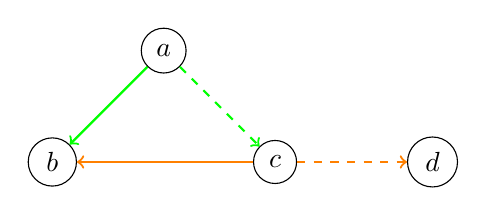
\begin{tikzpicture}[
            node distance={20mm},
            main/.style = {draw, circle},
            s/.style = {->,thick},
            d/.style = {->,thick,dashed} ]
        \node[main] (b) {$b$};
        \node[main] (a) [above right of=b] {$a$};
        \node[main] (c) [below right of=a] {$c$};
        \node[main] (d) [right of=c] {$d$};
        \draw[thick,green,->] (a) -- (b);
        \draw[thick,green,->,dashed] (a) -- (c);
        \draw[thick,orange,->] (c) -- (b);
        \draw[thick,orange,->,dashed] (c) -- (d);
    \end{tikzpicture}
    \caption{ 
        شبکه‌ی ناقض ویژگی لیست سیاه
    }
    \label{fig:blacklist}
\end{figure}

برای پیدا کردن علت نقض شدن ویژگی لیست سیاه شبکه‌ی رسم شده در شکل
\ref{fig:blacklist}
را در نظر بگیرید.
در این شبکه سوییچ
$d$
در لیست‌ سیاه قرار دارد، بنابراین در هیچ لحظه نباید از
$a$
که ورودی شبکه است در دسترس باشد.
بنابراین در شبکه عدم دسترسی 
$a$
به 
$d$
را به عنوان ویژگی در نظر می‌گیریم.
در شبکه‌ی بالا ابتدا مسیر‌هایی که با خط پررنگ مشخص شده‌اند وجود دارند.
در ادامه هر یک از این مسیرها با مسیر‌های خط‌چین جایگزین می‌شوند.
فرض کنید به روز رسانی این مسیر‌ها توسط دو پردازه هم‌روند انجام می‌شود.
واضح است که اگر هر دوی این به‌روز رسانی‌ها انجام شوند دسترسی به سوییچی که در لیست سیاه قرار دارد ممکن می‌شود.
اکنون فرض کنید که از عبارات زیر برای توصیف این شبکه در نت‌کت پویا استفاده کنیم:
\begin{equation*}
    \begin{aligned}[c]
        P   & = p!1                             \\
        Q   & = q!1                             \\
        N   & = F \oplus p?1;N_p \oplus q?1;N_q \\
        N_p & = F_p \oplus q?1;F_{pq}           \\
        N_q & = F_q \oplus p?1;F_{pq}           \\
        F   & = a\ra b \oplus c\ra b            \\
    \end{aligned}
    \qquad\qquad
    \begin{aligned}[c]
        F_p         & = a\ra c \oplus c\ra b \oplus a\ra b \\
        F_q         & = a\ra b \oplus c\ra d               \\
        F_{pq}      & = a\ra c \oplus c\ra d \oplus a\ra d \\
        SDN         & = \delta_{\mathcal{L}} (N
        \parallel P \parallel Q)                           \\
        \mathcal{L} & = \s{p!1,p?1,q?1,q?1}                \\
    \end{aligned}
\end{equation*}
در توصیف بالا پردازه‌های
$P$
و
$Q$
به ترتیب وظیفه‌ای ارسال پیام برای به روز رسانی مسیر‌های سبز و نارنجی را دارند.
پردازه‌ی
$N$
رفتار ابتدایی شبکه و پردازه‌های
$N_p$
و
$N_q$
به ترتیب رفتار شبکه را پس از به روز رسانی مسیر‌های سبز و نارنجی توصیف می‌کنند.
پردازه‌ های
$F,F_p,F_q,F_{pq}$
رفتارهای ارسالی%
\lf{Forwarding}
شبکه را توصیف می‌کنند.
در نهایت رفتار کلی شبکه توسط پردازه‌ی
$SDN$
توصیف شده است که حاصل ترکیب موازی پردازه‌های
$N,P,Q$
و جلوگیری از اجرای عملیات‌های همگام نشده است.
\begin{figure}
    \centering
    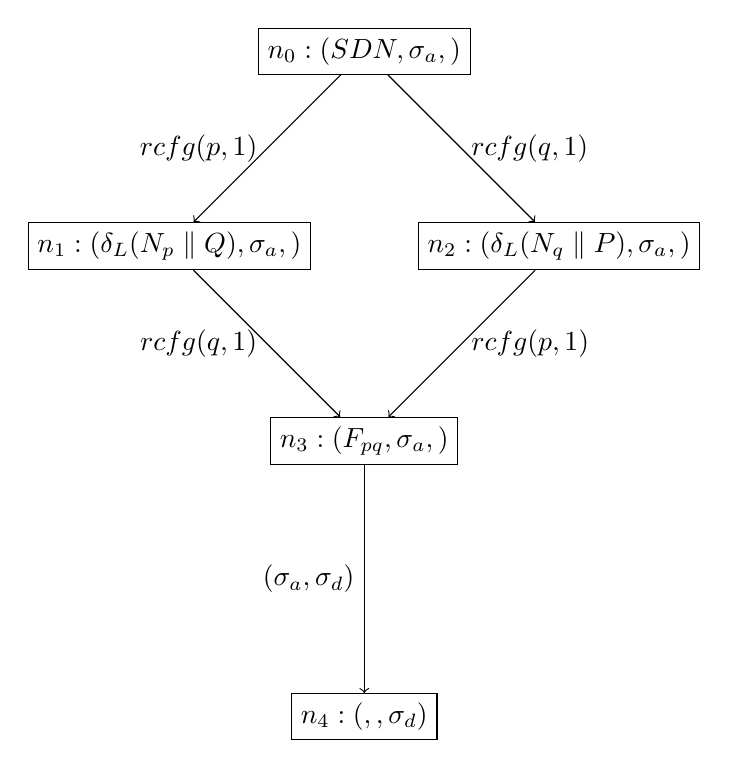
\begin{tikzpicture}[node distance={35mm},
            s/.style = {draw, rectangle,minimum width=5mm} ]
        \node[s] (n0) {$n_0: (SDN,\sigma_a,\his{})$};
        \node[s] (n1) [below left of=n0]
        {$n_1: (\delta_{\mc{L}}(N_p \parallel Q),\sigma_a,\his{})$};
        \node[s] (n3) [below right of=n1]
        {$n_3: (F_{pq},\sigma_a,\his{})$};
        \node[s] (n4) [below of=n3]
        {$n_4:(\checkmark,\his{},\sigma_d)$};
        \node[s] (n2) [below right of=n0]
        {$n_2: (\delta_{\mc{L}}(N_q \parallel P),\sigma_a,\his{}$)};
        \draw[->] (n0) -- node[left]{$rcfg(p,1)$} (n1);
        \draw[->] (n0) -- node[right]{$rcfg(q,1)$} (n2);
        \draw[->] (n1) -- node[left]{$rcfg(q,1)$} (n3);
        \draw[->] (n2) -- node[right]{$rcfg(p,1)$} (n3);
        \draw[->] (n3) -- node[left]{$(\sigma_a,\sigma_d)$} (n4);
    \end{tikzpicture}
    \caption{
        بخشی از سیستم انتقال 
        $SDN$
    }
    \label{fig:blacklist:lts}
\end{figure}
در توصیف بالا امکان اجرای هر دو به روز رسانی وجود دارد
بنابراین شبکه این امکان را دارد که به حالتی برسد که مسیری از 
$a$
به
$d$
در آن وجود داشته باشد.
برای مثال فرض کنید که
$\sigma_a$
یک بسته وارد شده به شبکه باشد که داشته باشیم:
$\sigma_a(sw) = a$.
شکل
\ref{fig:blacklist:lts}
بخشی از نمودار سیستم انتقال این شبکه را زمانی که این بسته به شبکه وارد شود نشان می‌دهد.
اگر فرض کنیم
$\sigma_d$
بسته‌ای باشد که
$\sigma_d(sw) = d$
همانطور که در نمودار مشخص است دو مسیر به حالتی که بسته از سوییچ
$a$
به
$d$
برسد وجود دارد.
به دلیل هم‌روندی پردازه‌های
$P$
و
$Q$
دو ترتیب برای اجرای این به‌روز رسانی‌ها وجود دارد و به همین دلیل دو مسیر منجر به خطا در این شبکه وجود دارد.
اکنون می‌خواهیم علت بروز این خطا را پیدا کنیم.
فرض کنید
$\mr{E} = \sem{SDN}$
ساختمان رویداد این شبکه و
$\mc{M}$
مدل علی
$\mr{E}$
بر اساس مدل تعریف شده در
\ref{es-causal-model}
باشد.
در این مدل تابع متغیر
$PV$
را به صورت زیر تعریف می‌کنیم:
\begin{align*}
    \f{PV} & = \exists c \in \mc{F}(ES(\vec v)). \exists e \in c. l(e) = a\ra d
\end{align*}
تابع بالا رفتار نا امن را وجود پیکربندی‌ای که شامل رویدادی با برچسب 
$a \ra d$
باشد توصیف می‌کند.
با توجه به ترتیب اجرای به‌روز‌رسانی‌ها در شبکه دو رویداد برای هر یک از عملیات‌های
$rcfg(p,1)$،
$rcfg(q,1)$
و
$a \ra d$
در ساختمان رویداد وجود دارد.
فرض کنید برای رویداد‌های مرتبط با این عملیات‌ها شش رویداد
$p_1,p_2,q_1,q_2,ad_1,ad_2$
وجود داشته باشد که برچسب آن‌ها به صورت زیر باشد:
\begin{align*}
    l(p_1) & = rcfg(p,1) \\
    l(p_2) & = rcfg(p,1) \\
    l(q_1) & = rcfg(q,1) \\
    l(q_2) & = rcfg(q,1) \\
    l(ad_1) & = a \ra d \\
    l(ad_2) & = a \ra d 
\end{align*}

\begin{figure}
    \centering
    \begin{tikzpicture}
        \crd{0}{0}{$\emptyset$}
        \crd[left]{-2}{1}{$\s{p_1}$}
        \crd[left]{-2}{2}{$\s{p_1,q_1}$}
        \crd[left]{-2}{3}{$\s{p_1,q_1,ad_1}$}
        \crd[right]{2}{1}{$\s{q_2}$}
        \crd[right]{2}{2}{$\s{p_2,q_2}$}
        \crd[right]{2}{3}{$\s{p_2,q_2,ad_2}$}
        \draw [ultra thick] (-2,1) -- (-2,2);
        \draw [ultra thick] (-2,2) -- (-2,3);
        \draw [ultra thick] (0,0) -- (2,1);
        \draw [ultra thick] (0,0) -- (-2,1);
        \draw [ultra thick] (2,1) -- (2,2);
        \draw [ultra thick] (2,1) -- (2,3);
    \end{tikzpicture}
    \caption{
        بخشی از پیکربندی‌های 
        ساختمان رویداد
        $SDN$
    }
    \label{fig:blacklist:es}
\end{figure}

شکل
\ref{fig:blacklist:es}
قسمتی از نمودار ساختمان رویداد این شبکه را نشان می‌دهد که در آن تمام پیکر‌بندی‌هایی که یکی از رویداد‌های 
$ad_1$
یا
$ad_2$
را داشته باشند
قابل دسترس باشد.
با استفاده از مدل علّی در این مثال می‌توانیم
$C(p_1,q_1) = \F$
را به عنوان یک علت برای نقض ویژگی لیست سیاه معرفی کنیم در صورتی که از
$(C(p_2,q_2),\T,\T)$
به عنوان شاهد استفاده کنیم.
ابتدا با توجه به شکل
\ref{fig:blacklist:es}
در 
$\mr{E}$
پیکربندی 
$\s{p_1,q_1,ad_1}$
قابل دسترسی است.
بنابراین مقدار
$PV$
صحیح است.
همچنین بین رویداد‌های 
$p_1$
و
$q_1$
تعارضی وجود ندارد پس داریم
$C(p_1,q_1) = \F$.
بنابراین شرط ۱ در تعریف 
\ref{def:extended}
برقرار است.

اکنون فرض کنید که مقدار
$C(p_1,q_1)$
و
$C(p_2,q_2)$
را برابر صحیح قرار دهیم.
در این حالت هیچ یک از پیکر‌بندی‌های 
$\s{p_1,q_1,ad_1}$
و
$\s{p_2,q_2,ad_2}$
دیگر نمی‌توانند عضوی از پیکربندی‌های 
$ES(\vec v)$
در 
$\mc{M}$
باشند زیرا با توجه به مقدار متغیر‌ها
بین روید‌اد‌های 
$p_1$
و
$q_1$
و همچنین بین رویداد‌های 
$p_2$
و
$q_2$
تعارض وجود دارد.
پس تحت این شرایط مقدار
$PV$
غلط می‌شود بنابراین شرط 
۲.آ هم برقرار می‌شود.
برای بررسی برقراری شرط ۲.ب
باید فرض کنیم که مقدار
$C(p_1,q_1)$
غلط است.
توجه کنید که در این شرایط پیکربندی
$\s{p_1,q_1,ad_1}$
عضوی از پیکربندی‌های 
$ES(\vec v)$
است و مقدار
$C(p_2,q_2)$
روی این مساله تاثیری ندارد.
همچنین برگرداندن مقادیر بقیه متغیر‌ها به مقدار اولیه آن‌ها باعث حذف 
$\s{p_1,q_1,ad_1}$
از مجموعه‌ی پیکربندی‌ها نمی‌شود بنابراین شرط ۲.ب هم برقرار است.
با توجه به اینکه علت تنها شامل یک جمله است بنابراین شرط مینیمال بودن هم برقرار است.
بنابراین در نهایت می‌توان نتیجه گرفت که 
$C(p_1,q_1)$
یک علت واقعی برای بروز خطا در این شبکه است.
در این مثال مشخص است که علت پیدا شده با علتی که به صورت شهودی باعث بروز خطا بوده است تطبیق دارد.



\section{نبود دور}
این ویژگی بیان می‌کند که شبکه‌ نباید هرگز دارای دور باشد
\cite{foerster2018survey}.
وجود دور در شبکه می‌تواند باعث مشکلاتی مانند دور زدن یک بسته در شبکه بدون رسیدن به مقصد و در نتیجه کاهش کارایی شبکه شود.
\begin{figure}
    \centering
    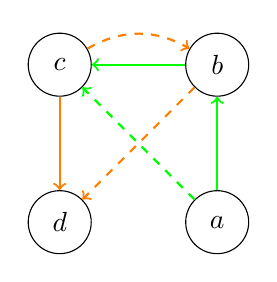
\begin{tikzpicture}[node distance={20mm},main/.style = {draw, circle,minimum size=8mm}]
        \node[main] (a)  {$a$};
        \node[main] (b) [above of=a]  {$b$};
        \node[main] (c) [left of=b] {$c$};
        \node[main] (d)  [below of=c] {$d$};
        \draw [->,green,thick] (a) -- (b);
        \draw [->,green,thick] (b) -- (c);
        \draw [->,orange,thick] (c) -- (d);
        \draw [->,green,thick,dashed] (a) -- (c);
        \draw [->,orange,thick,dashed] (c) edge[bend left] (b);
        \draw [->,orange,thick,dashed] (b) -- (d);
    \end{tikzpicture}
    \caption{ }
    \label{fig:loop}
\end{figure}
به عنوان مثال شبکه‌ی رسم شده در شکل
\ref{fig:loop}
را در نظر بگیرید.
در ابتدا مسیری از
$a$
به
$d$
وجود دارد.
در این شبکه دو به روز رسانی بر روی سوییچ‌های
$a$
و
$c$
انجام می‌شود تا مسیر جدیدی از
$a$
به
$d$
ایجاد شود که اینبار ابتدا از
$c$
عبور می‌کند.
می‌توانیم از توصیف نت‌کت پویای زیر برای توصیف این شبکه استفاده کنیم:
\begin{equation*}
    \begin{aligned}
        P           & = p!1                                             \\
        Q           & = q!1                                             \\
        N           & = F \oplus p?1;N_p \oplus q?1;N_q                 \\
        N_p         & = F_p \oplus q?1;F                                \\
        N_q         & = F_q \oplus p?1;F                                \\
        SDN         & = \delta_{\mathcal{L}}(N \parallel P \parallel Q) \\
        \mathcal{L} & = \s{p!1,p?1,q!1,q?1}
    \end{aligned}
    \qquad \qquad
    \begin{aligned}
        F    = & a\ra b \oplus a\ra c \oplus a\ra d               \\
               & \oplus b\ra c \oplus b\ra d \oplus c\ra d        \\
        F_p  = & a\ra c \oplus a\ra d \oplus c\ra d               \\
        F_q  = & a\ra b \oplus a\ra c \oplus a\ra d               \\
               & \oplus b\ra c \oplus b\ra b \oplus b\ra d        \\
               & \oplus        c\ra b \oplus c\ra c \oplus c\ra d
    \end{aligned}
\end{equation*}
در توصیف بالا پردازه‌های
$P$
و
$Q$
به ترتیب وظیفه‌ای ارسال پیام برای به روز رسانی مسیر‌های سبز و نارنجی را دارند.
توجه کنید که در این توصیف پس از اجرای هر دو به روزرسانی رفتار ارسالی شبکه همانند رفتار اولیه خود می‌شود.
همانطور که در شکل
\ref{fig:loop}
مشخص است اگر به روز رسانی نارنجی پیش از به روز رسانی سبز انجام شود در شبکه یک دور شامل گره‌های
$c$
و
$b$
ایجاد می‌شود.
\begin{figure}
    \centering
    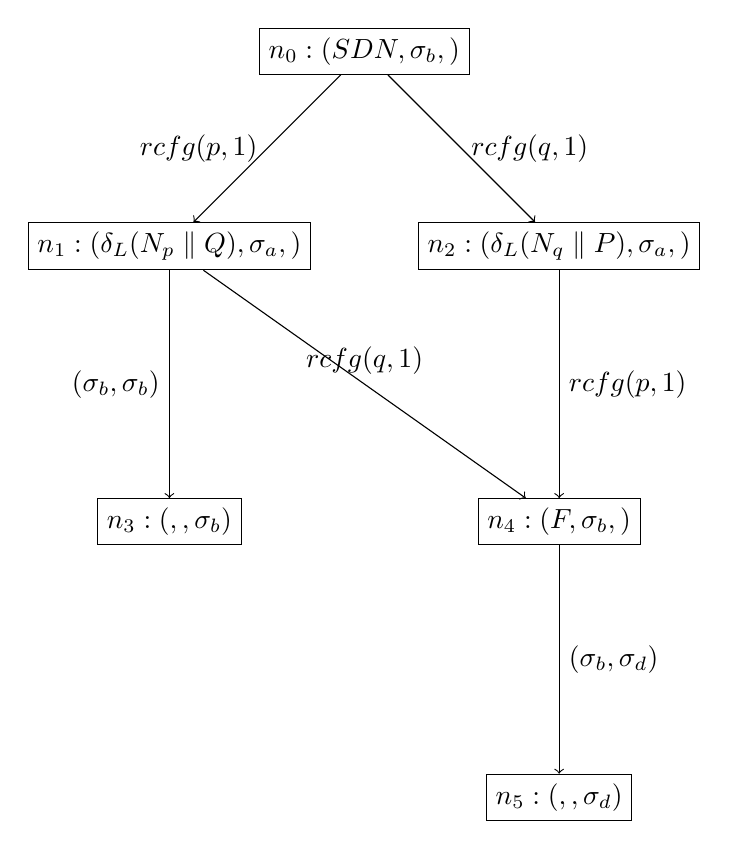
\begin{tikzpicture}[node distance={35mm},
            s/.style = {draw, rectangle,minimum width=5mm} ]
        \node[s] (n0) {$n_0: (SDN,\sigma_b,\his{})$};
        \node[s] (n1) [below left of=n0]
        {$n_1: (\delta_{\mc{L}}(N_p \parallel Q),\sigma_a,\his{})$};
        \node[s] (n3) [below of=n1]
        {$n_3: (\checkmark,\his{},\sigma_b)$};
        \node[s] (n2) [below right of=n0]
        {$n_2: (\delta_{\mc{L}}(N_q \parallel P),\sigma_a,
                \his{})$};
        \node[s] (n4) [below of=n2]
        {$n_4:(F,\sigma_b,\his)$};
        \node[s] (n5) [below of=n4]
        {$n_5:(\checkmark,\his{},\sigma_d)$};
        \draw[->] (n0) -- node[left]{$rcfg(p,1)$} (n1);
        \draw[->] (n0) -- node[right]{$rcfg(q,1)$} (n2);
        \draw[->] (n1) -- node[left]{$(\sigma_b,\sigma_b)$} (n3);
        \draw[->] (n1) -- node[above]{$rcfg(q,1)$} (n4);
        \draw[->] (n2) -- node[right]{$rcfg(p,1)$} (n4);
        \draw[->] (n4) -- node[right]{$(\sigma_b,\sigma_d)$} (n5);
    \end{tikzpicture}
    \caption{}
    \label{fig:loop:lts}
\end{figure}
شکل
\ref{fig:loop:lts}
قسمتی از سیستم انتقال برچسب‌دار شبکه را در حالتی که یک بسته ورودی روی سوییچ
$b$
وجود داشته باشد را نشان می‌دهد.
همانطور که در شکل مشخص است پس از انجام به روز رسانی مسیر نارنجی امکان عملیاتی به شکل
$(\sigma_b,\sigma_b)$
وجود دارد که به معنی وجود حلقه در این شبکه است.
اما اگر به روز رسانی مسیر سبز هم انجام شود تنها عملیات ممکن روی بسته ارسال آن به سوییچ
$d$
است.
اکنون فرض کنید که
$\mr{E} = \sem{SDN}$
ساختمان رویداد این شبکه و
$\mc{M}$
مدل علی
$\mr{E}$
بر اساس تعریف
باشد.
در این مدل تابع متغیر
$PV$
را به صورت زیر تعریف می‌کنیم:
\begin{align*}
    \f{PV} & = \bigvee_{c \in C} c \in \mathcal{F}(ES(\vec v)) \\
    C      & = \s{c \subset E | \exists e \in c.
        l(e) = b\ra b \vee l(e) = c\ra c }
\end{align*}
در این تابع رفتار نا امن وجود پیکربندی‌ای شامل یکی از برچسب‌های
$b \ra b$
یا
$c \ra c$
در شبکه است.
همانند مثال قبل با توجه به ترتیب اجرای به‌روز‌رسانی‌ها در شبکه دو رویداد برای هر یک از عملیات‌های
$rcfg(p,1)$
و
$rcfg(q,1)$
در ساختمان رویداد وجود دارد.
فرض کنید برای رویداد‌های مرتبط با این عملیات‌ها چهار رویداد
$p_1,p_2,q_1,q_2$
وجود داشته باشد که برچسب آن‌ها به صورت زیر باشد:
\begin{align*}
    l(p_1) & = rcfg(p,1) \\
    l(p_2) & = rcfg(p,1) \\
    l(q_1) & = rcfg(q,1) \\
    l(q_2) & = rcfg(q,1)
\end{align*}
همچنین فرض کنید برچسب رویداد‌های
$bb,cc$
به ترتیب
$b\ra b,c\ra c$
باشد.
\begin{figure}
    \centering
    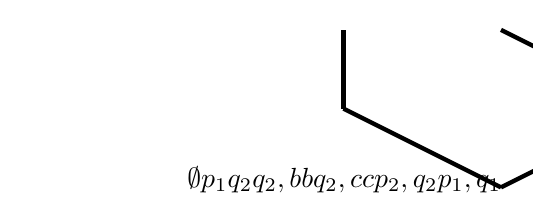
\begin{tikzpicture}
        \crd{0}{0}{$\emptyset$}
        \crd[below]{-2}{1}{$\s{p_1}$}
        \crd[below]{2}{1}{$\s{q_2}$}
        \crd[above]{2}{2}{$\s{q_2,bb}$}
        \crd[above]{4}{2}{$\s{q_2,cc}$}
        \crd[above]{0}{2}{$\s{p_2,q_2}$}
        \crd[left]{-2}{2}{$\s{p_1,q_1}$}
        \draw [ultra thick] (0,0) -- (2,1);
        \draw [ultra thick] (0,0) -- (-2,1);
        \draw [ultra thick] (2,1) -- (0,2);
        \draw [ultra thick] (2,1) -- (2,2);
        \draw [ultra thick] (2,1) -- (4,2);
        \draw [ultra thick] (-2,1) -- (-2,2);
    \end{tikzpicture}
    \caption{}
    \label{fig:loop:es}
\end{figure}
شکل
\ref{fig:loop:es}
قسمتی از نمودار ساختمان رویداد این شبکه را نشان می‌دهد که در آن تمام پیکر‌بندی‌هایی وجود داشته باشد که یکی از رویداد‌های
$bb$
یا
$cc$
قابل دسترس باشد.

در این مثال می‌توان
$M_{\s{p_2},q_2}= \F$
با در نظر گرفتن
$(\e,\e,\T)$
به عنوان شاهد را یک علت واقعی وجود دور در این شبکه
معرفی کرد.
با توجه به تعریف مدل علّی در بخش
\ref{es-causal-model}
توابع متغیر‌های
$M_{\e,q_2}$
و
$EN_{\e,q_2}$
به صورت زیر تعریف می‌شوند:
\begin{align*}
    \f{M_{\e,q_2}}  & = Min(\e,q_2) \wedge Con(\e) \\
                    & = Min(\e,q_2)                \\
                    & =  \bigwedge_{q_2 \notin s'}
    \neg M_{s',q_2}                                \\
    \f{EN_{\e,q_2}} & = M_{\e,q_2}
\end{align*}
با توجه به این توابع واضح است که 
اگر مقدار
$M(\s{p_2},q_2)$
را برابر صحیح قرار دهیم آنگاه مقدار
$M(\e,q_2)$
غلط شده و در نتیجه مقدار
$EN(\e,q_2)$
هم غلط می‌شود.
برای اینکه هر کدام از مجموعه‌های شاخه‌ی راست شکل
\ref{fig:loop:es}
عضوی از مجموعه‌ی پیکربندی‌های 
$ES(\vec v)$
باشند باید داشته باشیم:
$\e \vdash q_2$
اما با توجه به این مقدار متغیر متناظر با این رابطه غلط شده است بنابراین این رابطه در 
$ES(\vec v)$
وجود ندارد، پس هیچ کدام از این مجموعه‌ها عضوی از پیکربندی‌های 
$ES(\vec v)$
نیستند.
بنابراین در این شرایط مقدار متغیر 
$PV$
غلط شده و شرط ۲.آ در تعریف 
\ref{def:extended}
برقرار می‌شود.
با توجه به گزاره‌ی 
\ref{prop:but-for}
چون
$\vec W$
در شاهد خالی است می‌توان نتیجه گرفت که
$M(\s{p_2},q_2) = \F$
علت واقعی به وجود آمدن دور در این شبکه است.


\section{نبود سیاه‌چاله}
در یک شبکه سیاه‌چاله‌ها%
\lf{Blackhole}
عناصری در شبکه هستند که وظیفه ارسال بسته‌ها را دارند
(مثلا سوییچ‌ یا روتر)
ولی برخی از بسته‌ها را پس از دریافت به جایی ارسال نمی‌کنند و در واقع مانند سیاه‌چاله این بسته‌ها در آن‌ها گم می‌شوند
\cite{network-abstractions}.
در یک شبکه که مکان‌های ورودی و خروجی مشخص دارد عدم وجود سیاه‌چاله در شبکه را می‌توان معادل این ويژگی که همه‌ی بسته‌های ورودی به شبکه از آن خارج شوند دانست.
\begin{figure}
    \centering
    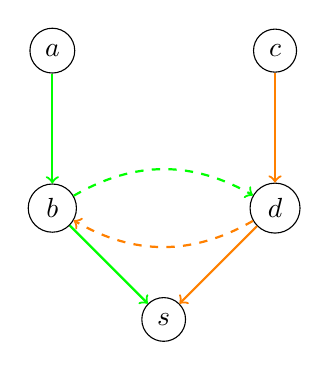
\begin{tikzpicture}[
            node distance={20mm},
            main/.style = {draw, circle},
            s/.style = {->,thick},
            d/.style = {->,thick,dashed} ]
        \node[main] (s) {$s$};
        \node[main] (b) [above left of=s] {$b$};
        \node[main] (a) [above of=b] {$a$};
        \node[main] (d) [above right of=s] {$d$};
        \node[main] (c) [above of=d] {$c$};
        \draw[thick,green,->] (a) -- (b);
        \draw[thick,green,->] (b) -- (s);
        \draw[thick,green,->,dashed] (b) edge[bend left] (d);
        \draw[thick,orange,->] (c) -- (d);
        \draw[thick,orange,->] (d) -- (s);
        \draw[thick,orange,->,dashed] (d) edge[bend left] (b);
    \end{tikzpicture}
    \caption{ 
        شبکه‌ی ناقض ویژگی نبود سیاه‌چاله
    }
    \label{fig:blackhole}
\end{figure}
به عنوان مثال شبکه‌ی موجود در شکل
\ref{fig:blackhole}
را در نظر بگیرید.
فرض کنید که در این شبکه
$a,c$
ورودی‌های شبکه و
$s$
خروجی شبکه باشد.
در این شبکه دو به روز رسانی برای جایگزینی
مسیر
$ds$
با
$db$
و مسیر
$bs$
با
$bd$
انجام می‌شود.
در این شبکه در حالت ابتدایی و پس از انجام یکی از به روز‌رسانی‌ها ورودی‌ها به خروجی مسیر وجود دارد اما اگر هر دوی این به روز رسانی‌ها انجام شوند دیگر
$s$
قابل دسترسی نیست و عملا بسته‌های ورودی به شبکه به خروجی نمی‌رسند.
این شبکه را می‌توانیم به فرم زیر در نت‌کت پویا توصیف کنیم:
\begin{equation*}
    \begin{aligned}[c]
        P   & = p!1                             \\
        Q   & = q!1                             \\
        N   & = F \oplus p?1;N_p \oplus q?1;N_q \\
        N_p & = F \oplus q?1;F_{pq}             \\
        N_q & = F \oplus p?1;F_{pq}
    \end{aligned}
    \qquad\qquad
    \begin{aligned}[c]
        F           & = a\ra s \oplus c\ra s            \\
        F_{pq}      & = a\ra b \oplus c\ra d            \\
        SDN         & = \delta_{\mathcal{L}} (N
        \parallel P \parallel Q)                \\
        \mathcal{L} & = \s{p!1,p?1,q?1,q?1}
    \end{aligned}
\end{equation*}
در ادامه فرض کنید که 
$\mc{M}$
مدل علّی این شبکه باشد.
در این مدل تابع متغیر
$PV$
را به صورت زیر تعریف می‌کنیم:
\begin{align*}
    \f{PV} & = \exists c \in \mathcal{F}(ES(\vec v)),
    \exists e \in c. l(e) =  \alpha\cdot\pi \wedge \pi(sw) \neq s
\end{align*}
در تعریف این تابع رفتار نا امن وجود یک پیکربندی شامل رویدادی با برچسب از نوع 
$\alpha \cdot \pi$
یا به عبارت دیگر رویدادی از نوع ارسال بسته است که سوییچ مقصد ارسال آن سوییچ 
$s$
نباشد.
همانند مثال مربوط نبود دور در شبکه، در این مثال هم با توجه به ترتیب اجرای به روز رسانی‌ها دو رویداد برای هر یک از عملیات‌های 
$rcfg(p,1)$
،$rcfg(q,1)$
و
$a\ra b,a c\ra d$
وجود دارد. 
بنابراین فرض کنید که رویدادهای
$p_i,q_i,ab_i,cd_i$
به ازای 
$i=1,2$
در ساختمان رویداد این مدل وجود داشته باشند و برچسب‌گذاری آن‌ها به صورت زیر باشد:
\begin{align*}
    l(p_1) & = rcfg(p,1) \\
    l(p_2) & = rcfg(p,1) \\
    l(q_1) & = rcfg(q,1) \\
    l(q_2) & = rcfg(q,1) \\
    l(ab_1) & = a \ra b \\
    l(ab_2) & = a \ra b \\
    l(cd_1) & = c \ra d \\
    l(cd_2) & = c \ra d \\
\end{align*}
\begin{figure}
    \centering
    \begin{tikzpicture}
        \crd{0}{0}{$\emptyset$}
        \crd[left]{-2}{1}{$\s{p_1}$}
        \crd[left]{-2}{2}{$\s{p_1,q_1}$}
        \crd[above]{-1}{3}{$\s{p_1,q_1,ab_1}$}
        \crd[left]{-3}{3}{$\s{p_1,q_1,cd_1}$}
        \crd[right]{2}{1}{$\s{q_2}$}
        \crd[right]{2}{2}{$\s{p_2,q_2}$}
        \crd[above]{1}{3}{$\s{p_2,q_2,ab_2}$}
        \crd[right]{3}{3}{$\s{p_2,q_2,cd_2}$}
        \draw [ultra thick] (-2,1) -- (-2,2);
        \draw [ultra thick] (-2,2) -- (-1,3);
        \draw [ultra thick] (-2,2) -- (-3,3);
        \draw [ultra thick] (0,0) -- (2,1);
        \draw [ultra thick] (0,0) -- (-2,1);
        \draw [ultra thick] (2,1) -- (2,2);
        \draw [ultra thick] (2,2) -- (1,3);
        \draw [ultra thick] (2,2) -- (3,3);
    \end{tikzpicture}
    \caption{
        بخشی از پیکربندی‌های ساختمان رویداد
        $SDN$
    }
    \label{fig:blackhole:es}
\end{figure}
پیکربندی‌هایی از این ساختمان رویداد که شامل رویدادی با برچسب 
$a \ra b$
یا 
$c \ra d$
باشند نقض شدن ویژگی نبود سیاه‌چاله را نشان می‌دهند.
بنابراین تابع متغیر
$PV$
را به فرم زیر توصیف می کنیم:
\begin{align*}
    \f{PV} & = \exists c \in \mathcal{F}(ES(\vec v)),
    \exists e \in c. l(e) =  \alpha\cdot\pi \wedge \pi(sw) \neq s
\end{align*}
در این مدل هم همانند مثال نبود دور در شبکه عدم وجود تعارض بین رویداد‌های 
$p_1$
و
$q_1$
را می‌توان به عنوان علت واقعی نقض شدن ویژگی در نظر گرفت.
برای این منظور از شاهد
$(C_{p_2,q_2},\T,\T)$
استفاده می‌کنیم.
واضح است که اگر مقدار هر دو متغیر
$C_{p_1,q_1}$
و
$C_{p_2,q_2}$
را برابر غلط قرار دهیم آنگاه هیچ یک از پیکر‌بندی‌های 
$\s{p_1,q_1,cd_1},\s{p_1,q_1,ab_1},\s{p_2,q_2,ab_2},\s{p_2,q_2,cd_2}$
دیگر عضوی از پیکربندی‌های 
$ES(\vec v)$
نیستند.
از طرفی در شرایطی که 
$C_{p_1,q_1}$
مقدار درست داشته باشد آنگاه پیکربندی‌های
$\s{p_1,q_1,ab_1},\s{p_1,q_1,cd_1}$
عضو
$ES(\vec v)$
هستند و مقدار متغیر
$C_{p_2,q_2}$
تاثیری روی این مساله ندارد بنابراین در نهایت می‌توان نتیجه گرفت که 
$C_{p_1,q_1} = \F$
علت واقعی نقض ویژگی است.

% \section{کنترل ازدحام}
برای کنترل ازدحام
\lf{Congestion Control}
برخی از پیوند‌ها یا سوییچ‌های شبکه ظرفیت مشخصی دارند و به همین دلیل جریان
\lf{Flow}
عبوری از آن‌ها نباید از ظرفیت آن‌ها بیشتر شود.

\begin{figure}
    \centering
    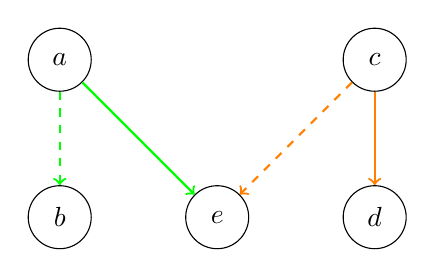
\begin{tikzpicture}[node distance={20mm},main/.style = {draw, circle,minimum size=8mm}]
        \node[main] (a)  {$a$};
        \node[main] (b) [below of=a]  {$b$};
        \node[main] (e) [right of=b] {$e$};
        \node[main] (d)  [right of=e] {$d$};
        \node[main] (c) [above of=d] {$c$};
        \draw [->,green,thick,dashed] (a) -- (b);
        \draw [->,orange,thick] (c) -- (d);
        \draw [->,green,thick] (a) -- (e);
        \draw [->,orange,thick,dashed] (c) -- (e);
    \end{tikzpicture}
    \caption{ 
        شبکه‌ی ناقض ویژگی عدم ازدحام
    }
    \label{fig:congestion}
\end{figure}
به عنوان مثال شبکه‌ی رسم شده در شکل
\ref{fig:congestion}
را در نظر بگیرید.
در این شبکه فرض کنید که سوییچ‌های
$a$
،
$c$
و
$e$
ظرفیت پردازش حداکثر یک بسته در هر ثانیه را داشته باشند.
در این شبکه ابتدا مسیری از
$a$
به
$e$
و از
$c$
به
$d$
وجود دارد و دو به روز رسانی بر روی سوییچ‌های
$a$
و
$c$
این مسیر‌ها را با مسیر‌های
$ab$
و
$cd$
جایگزین می‌کند.
این شبکه را می‌توانیم به شکل زیر در نت‌کت پویا توصیف کنیم:
\begin{equation*}
    \begin{aligned}[c]
        P   & = p!1                               \\
        Q   & = q!1                               \\
        N   & = F^2 \oplus p?1;N_p \oplus q?1;N_q \\
        N_p & = F_p^2 \oplus q?1;F_{pq}^2         \\
        N_q & = F_q^2 \oplus p?1;F_{pq}^2         \\
        F   & = a\ra b \oplus c\ra d                      \\
    \end{aligned}
    \qquad
    \begin{aligned}[c]
        F_p         & = a\ra e \oplus c\ra d         \\
        F_q         & = c\ra e \oplus a\ra b         \\
        F_{pq}      & = a\ra e \oplus c\ra e         \\
        SDN         & = \delta_{\mathcal{L}}
        (N \parallel P \parallel Q)          \\
        \mathcal{L} & = \s{p!1,p?1,q!1,q?1}
    \end{aligned}
\end{equation*}
در توصیف بالا پردازه‌های
$P$
و
$Q$
به ترتیب وظیفه‌ای ارسال پیام برای به روز رسانی مسیر‌های سبز و نارنجی را دارند.
برای ساده شدن این مثال، شبکه را به گونه‌ای توصیف کرده‌ایم که توانایی پردازش حداکثر دو بسته را داشته باشد.
در این توصیف از عباراتی به فرم
$F^2$
برای نشان دادن 
$F;F$
استفاده شده است.
\begin{figure}
    \centering
    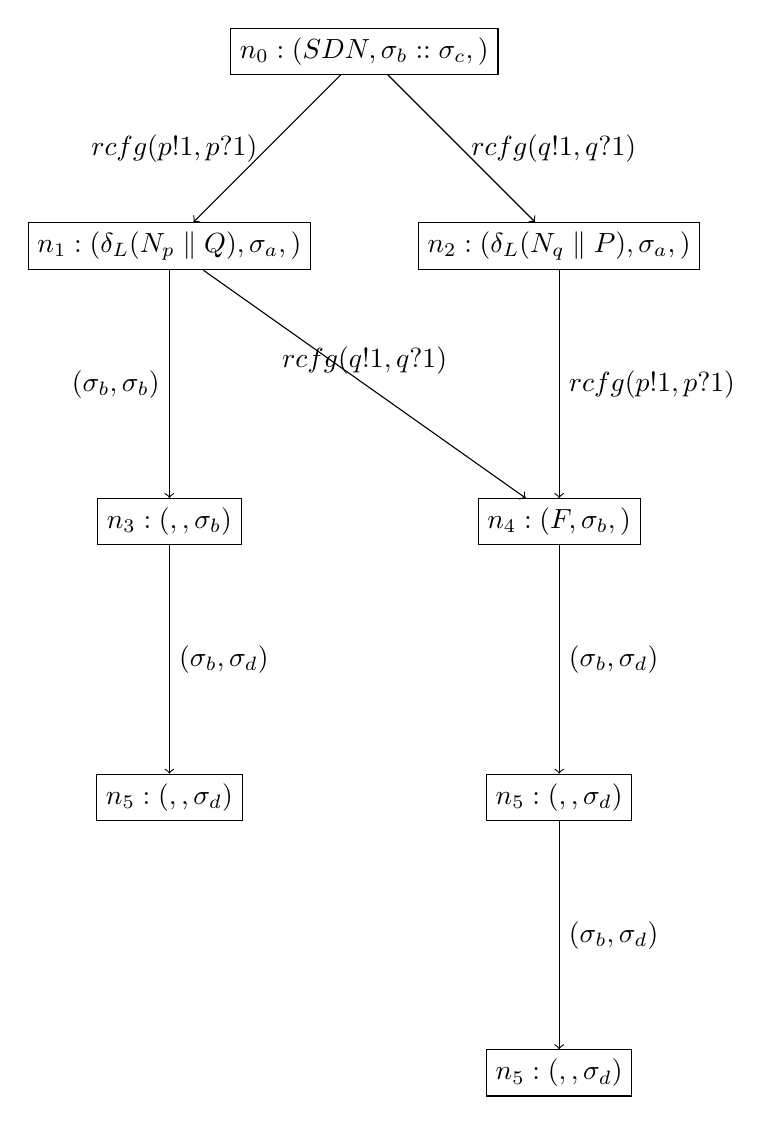
\begin{tikzpicture}[node distance={35mm},
            s/.style = {draw, rectangle,minimum width=5mm} ]
        \node[s] (n0) {$n_0: (SDN,\sigma_b::\sigma_c,\his{})$};
        \node[s] (n1) [below left of=n0]
        {$n_1: (\delta_{\mc{L}}(N_p \parallel Q),\sigma_a,\his{})$};
        \node[s] (n3) [below of=n1]
        {$n_3: (\checkmark,\his{},\sigma_b)$};
        \node[s] (n2) [below right of=n0]
        {$n_2: (\delta_{\mc{L}}(N_q \parallel P),\sigma_a,
                \his{})$};
        \node[s] (n4) [below of=n2]
        {$n_4:(F,\sigma_b,\his)$};
        \node[s] (n5) [below of=n3]
        {$n_5:(\checkmark,\his{},\sigma_d)$};
        \node[s] (n6) [below of=n4]
        {$n_5:(\checkmark,\his{},\sigma_d)$};
        \node[s] (n7) [below of=n6]
        {$n_5:(\checkmark,\his{},\sigma_d)$};
        \draw[->] (n0) -- node[left]{$rcfg(p!1,p?1)$} (n1);
        \draw[->] (n0) -- node[right]{$rcfg(q!1,q?1)$} (n2);
        \draw[->] (n1) -- node[left]{$(\sigma_b,\sigma_b)$} (n3);
        \draw[->] (n1) -- node[above]{$rcfg(q!1,q?1)$} (n4);
        \draw[->] (n2) -- node[right]{$rcfg(p!1,p?1)$} (n4);
        \draw[->] (n4) -- node[right]{$(\sigma_b,\sigma_d)$} (n6);
        \draw[->] (n6) -- node[right]{$(\sigma_b,\sigma_d)$} (n7);
        \draw[->] (n3) -- node[right]{$(\sigma_b,\sigma_d)$} (n5);
    \end{tikzpicture}
    \caption{}
    \label{fig:congestion:lts}
\end{figure}
شکل
\ref{fig:congestion:lts}
قسمتی از سیستم انتقال برچسب‌دار شبکه را در حالتی که یک بسته ورودی روی سوییچ
$b$
وجود داشته باشد را نشان می‌دهد.
همانطور که در شکل مشخص است پس از انجام به روز رسانی مسیر نارنجی امکان عملیاتی به شکل
$(\sigma_b,\sigma_b)$
وجود دارد که به معنی وجود حلقه در این شبکه است.
اما اگر به روز رسانی مسیر سبز هم انجام شود تنها عملیات ممکن روی بسته ارسال آن به سوییچ
$d$
است.
اکنون فرض کنید که
$\mr{E} = \sem{SDN}$
ساختمان رویداد این شبکه و
$\mc{M}$
مدل علی
$\mr{E}$
بر اساس تعریف
باشد.
در این مدل تابع متغیر
$PV$
را به صورت زیر تعریف می‌کنیم:
\begin{align*}
    \f{PV} & = \bigvee_{c \in C} c \in \mathcal{F}(ES(\vec v)) \\
    C      & = \s{c \subset E | \exists e \in c.
        l(e) = b\ra b \vee l(e) = c\ra c }
\end{align*}
در این تابع رفتار نا امن وجود پیکربندی‌ای شامل یکی از برچسب‌های
$b \ra b$
یا
$c \ra c$
در شبکه است.
همانند مثال قبل با توجه به ترتیب اجرای به‌روز‌رسانی‌ها در شبکه دو رویداد برای هر یک از عملیات‌های
$rcfg(p!1,p?1)$
و
$rcfg(q!1,q?1)$
در ساختمان رویداد وجود دارد.
فرض کنید برای رویداد‌های مرتبط با این عملیات‌ها چهار رویداد
$p_1,p_2,q_1,q_2$
وجود داشته باشد که برچسب آن‌ها به صورت زیر باشد:
\begin{align*}
    l(p_1) & = rcfg(p!1,p?1) \\
    l(p_2) & = rcfg(p!1,p?1) \\
    l(q_1) & = rcfg(q!1,q?1) \\
    l(q_2) & = rcfg(q!1,q?1)
\end{align*}
همچنین فرض کنید برچسب رویداد‌های
$bb,cc$
به ترتیب
$b\ra b,c\ra c$
باشد.
\begin{figure}
    \centering
    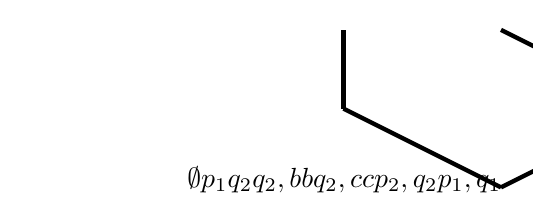
\begin{tikzpicture}
        \crd{0}{0}{$\emptyset$}
        \crd[below]{-2}{1}{$\s{p_1}$}
        \crd[below]{2}{1}{$\s{q_2}$}
        \crd[above]{2}{2}{$\s{q_2,bb}$}
        \crd[above]{4}{2}{$\s{q_2,cc}$}
        \crd[above]{0}{2}{$\s{p_2,q_2}$}
        \crd[left]{-2}{2}{$\s{p_1,q_1}$}
        \draw [ultra thick] (0,0) -- (2,1);
        \draw [ultra thick] (0,0) -- (-2,1);
        \draw [ultra thick] (2,1) -- (0,2);
        \draw [ultra thick] (2,1) -- (2,2);
        \draw [ultra thick] (2,1) -- (4,2);
        \draw [ultra thick] (-2,1) -- (-2,2);
    \end{tikzpicture}
    \caption{}
    \label{fig:loop:es}
\end{figure}
شکل
\ref{fig:loop:es}
قسمتی از نمودار ساختمان رویداد این شبکه را نشان می‌دهد که در آن تمام پیکر‌بندی‌هایی وجود داشته باشد که یکی از رویداد‌های
$bb$
یا
$cc$
قابل دسترس باشد.

در این مثال می‌توان
$M_{\s{p_2},q_2}= \F$
با در نظر گرفتن
$(\e,\e,\T)$
به عنوان شاهد را یک علت واقعی وجود دور در این شبکه
معرفی کرد.
با توجه به تعریف مدل علّی در بخش
\ref{es-causal-model}
توابع متغیر‌های
$M_{\e,q_2}$
و
$EN_{\e,q_2}$
به صورت زیر تعریف می‌شوند:
\begin{align*}
    \f{M_{\e,q_2}}  & = Min(\e,q_2) \wedge Con(\e) \\
                    & = Min(\e,q_2)                \\
                    & =  \bigwedge_{q_2 \notin s'}
    \neg M_{s',q_2}                                \\
    \f{EN_{\e,q_2}} & = M_{\e,q_2}
\end{align*}
با توجه به این توابع واضح است که
اگر مقدار
$M(\s{p_2},q_2)$
را برابر صحیح قرار دهیم آنگاه مقدار
$M(\e,q_2)$
غلط شده و در نتیجه مقدار
$EN(\e,q_2)$
هم غلط می‌شود.
برای اینکه هر کدام از مجموعه‌های شاخه‌ی راست شکل
\ref{fig:loop:es}
عضوی از مجموعه‌ی پیکربندی‌های
$ES(\vec v)$
باشند باید داشته باشیم:
$\e \vdash q_2$
اما با توجه به این مقدار متغیر متناظر با این رابطه غلط شده است بنابراین این رابطه در
$ES(\vec v)$
وجود ندارد، پس هیچ کدام از این مجموعه‌ها عضوی از پیکربندی‌های
$ES(\vec v)$
نیستند.
بنابراین در این شرایط مقدار متغیر
$PV$
غلط شده و شرط ۲.آ در تعریف
\ref{def:extended}
برقرار می‌شود.
با توجه به گزاره‌ی
\ref{prop:but-for}
چون
$\vec W$
در شاهد خالی است می‌توان نتیجه گرفت که
$M(\s{p_2},q_2) = \F$
علت واقعی به وجود آمدن دور در این شبکه است.

% \section{تعمیم ویژگی‌ها}
در این بخش چگونگی توصیف رفتار ناامن برای ویژگی‌های بررسی شده در بخش قبلی بیان می‌شود.

\subsection{بدون دور بودن}


